\documentclass[11pt]{report}
\usepackage[letterpaper, total={6.5in, 10in}]{geometry}
%\usepackage{fancyhdr}
%\pagestyle{fancy}
\usepackage{amsmath, amsthm, mathpazo, epic, eepic, color, array}
\usepackage{amssymb}
%\usepackage{graphicx}
\usepackage{cancel}
\usepackage{pgfplots}
\usepackage{multicol}
\pgfplotsset{compat=1.13}
\usepackage{etoolbox}
\makeatletter
\patchcmd{\chapter}{\if@openright\cleardoublepage\else\clearpage\fi}{}{}{}
\makeatother
\usepackage{hyperref}

\usepackage{enumerate}
\usepackage{enumitem}

\usepackage{tikz}
\usetikzlibrary{positioning,chains,fit,shapes,calc,arrows,patterns}
\usepackage{tkz-graph}
\usetikzlibrary{arrows, petri, topaths}
\usepackage{tkz-berge}
\usepackage[all]{xy}
\usepackage{textcomp}

\newboolean{colorprint}
\setboolean{colorprint}{true}
%\setboolean{colorprint}{false}

\ifthenelse{\boolean{colorprint}}{%
\newcommand{\colorone}{blue}
\newcommand{\colortwo}{red}
\newcommand{\coloronefill}{blue!15!white}
\newcommand{\colortwofill}{red!15!white}
\newcommand{\colormapone}{rgb=(.4,.4,1); rgb=(.8,.8,1)}
\newcommand{\colormaptwo}{rgb=(1,.4,.4); rgb=(1,.8,.8)}
\newcommand{\colormapplaneone}{rgb=(.7,.7,1); rgb=(.9,.9,1)}
\definecolor{colormaponebottom}{rgb}{.4,.4,1}
\definecolor{colormaponetop}{rgb}{.8,.8,1}
\definecolor{colormaptwobottom}{rgb}{1,.4,.4}
\definecolor{colormaptwotop}{rgb}{1,.8,.8}
}% ends color
{% not color
\newcommand{\colorone}{black}
\newcommand{\colortwo}{black!50!white}
\newcommand{\coloronefill}{black!15!white}
\newcommand{\colortwofill}{black!05!white}
\newcommand{\colormapone}{rgb=(.4,.4,.4); rgb=(.7,.7,.7)}
\newcommand{\colormaptwo}{rgb=(.6,.6,.6); rgb=(.9,.9,.9)}
\newcommand{\colormapplaneone}{rgb=(.8,.8,.8); rgb=(.95,.95,.95)}
\definecolor{colormaponebottom}{rgb}{.4,.4,.4}
\definecolor{colormaponetop}{rgb}{.7,.7,.7}
\definecolor{colormaptwobottom}{rgb}{.6,.6,.6}
\definecolor{colormaptwotop}{rgb}{.9,.9,.9}
}%

\newlength\tindent
\setlength{\tindent}{\parindent}
\setlength{\parindent}{0pt}
\renewcommand{\indent}{\hspace*{\tindent}}

\pgfplotsset{my style/.append style={axis x line=middle, axis y line=
middle, xlabel={$x$}, ylabel={$y$}, axis equal }}

\pgfplotsset{compat=1.13}

\usepackage[normalem]{ulem}

\begin{document}

{\bf Chapter 2: Derivatives}\\

%%%%%%%%%%%%%%%%%%%%%%Section 2.6%%%%%%%%%%%%%%%
{\bf Section 2.6 Implicit Differentiation}
\vskip .25 truein

All page numbers refer to original APEX text page numbers.\\
\\
In general, in this section, watch for the use of the word "function". \\

\textbf{p. 106} \\

Third paragraph: "... A graph of this implicit \sout{function} equation is given..."\\

The line with $\displaystyle{\frac{d}{dx}\left(f(y)\right)}$ needs to have  right ) parenthses removed in three places after the $f(y)$\\


\textbf{p. 107} \\

In the two paragraphs under the solution to Example 67: The word "function(s)" either needs to be replaced (or could just be replaced for consistency) with "equation(s)" in at least 6 places.\\

Example 68 change the directions to say: "Find the equation of the line tangent to the implicitly defined curve $y + y^3$..."\\

\textbf{pp. 108-109} \\

Toward the end of the solution to Example 68: Therefore the equation of... defined \sout{function} curve..."\\

Example 69 - replace the format of the current solution with:\\
\tiny \textbf{SOLUTION} \normalsize \hskip .5 truecm We will take the implicit derivatives term by term. Using the Chain Rule the derivative of $y^3$ is $3y^2 y'$.\\
\indent The second term, , $x^2y^4$ is a little more work. It requires the Product Rule as it is the product of two functions of $x$: $x^2$ and $y^4$. We see that $\displaystyle{\frac{d}{dx}(x^2y^4)}$ is\\
\begin{center}
$\displaystyle{x^2 \cdot \frac{d}{dx}(y^4) + \frac{d}{dx}(x^2) \cdot y^4}$\\
$\displaystyle{x^2 \cdot (4y^3y') + 2x \cdot y^4}$\\
\end{center}
\vskip .25 truecm
The first part of this expression requires a $y'$ because we are taking the derivative of a $y$ term. The second part does not require it because we are taking the derivative of $x^2$.\\
\indent The derivative of the right hand side of the equation is found to be $2$... \\

Top of page 109 - lots of "function" use -\\
\indent To confirm the validity of...to this \sout{function} curve at a point... graph of this \sout{function} curve... The \sout{function} equation and its tangent..."\\
\indent Notice how our curve looks much different than the graphs of functions we have worked with up to this point. \sout{It fails the vertical line test.}Such curves are important in many areas of mathematics, so develping tools to deal with them is important.\\
\\
Figure 2.21 description, replace "function" with "curve". Same for Figure 2.22 description.\\

Example 70:\\
"Given the implicitly defined \sout{function} curve..."\\

\textbf{p. 110} \\
First line replace "function" with "equation"\\
Tim, can you mess with the graph so we can see the 3rd tangent line - or is it just not possible? Maybe it could be made longer.\\

Second to the last paragrph: "This section has shown... defined \sout{functions} curves..."\\

\textbf{p. 110-112} \\
I think we decided to cut this everything from the last paragraph on p. 110  \sout{"One hole in ...}"
through Example 72 on p. 112. The proof will be given in Calculus II after discussion of logarithmic differentiation.

\textbf{p. 113} \\
Example 73 Solution:\\
After "replace $y'$ with $\frac{-x}{y}$:\\



\begin{flalign*}
\begin{aligned}
y'' &=\displaystyle{ -\frac{y-x \cdot \frac{-x}{y}}{y^2}}\\
&= \displaystyle{ -\frac{y+ \frac {x^2}{y}}{y^2}}\\
&= \displaystyle{ -\frac{y+\frac {x^2}{y}}{y^2}\cdot \frac{y}{y}}\\
&= \displaystyle{ -\frac{y^2+x^2}{y^3}}, \text{ since we were given } x^2 + y^2=1\\
&= \displaystyle{ -\frac{1}{y^3}}\\
\end{aligned}
\end{flalign*}
\vskip .25 truecm

\textbf{p. 113 - 114}\\
Move Logarithmic Differentiation section to Calculus II.

Create a Chapter Summary section to include a table of the derivatives developed in this chapter. The intro of this section can be the paragraph that currently appears right before Theorem 24. From Theorem 24 we want to include \#1-9, 13-18 in this table.
\vskip 1 truecm

\textbf{Exercises}\\
Cut exercises \#5 - 12 \& move \#18, 36-41 to the appropriate Calculus II sections\\

\textbf{After current \#25 insert the following 3 problems:}\\

$\displaystyle xe^x = ye^y$\\

\indent Answer: $\displaystyle y'=\frac{e^x(x+1)}{e^y(y+1)}$\vskip 1 truecm

$\displaystyle y\sin(x^3) = x\sin(y^3)$\\

\indent Answer: $\displaystyle y'=\frac{3x^2y\cos x^3 - \sin y^3}{3xy^2\sin y^3 - \sin x^3}$\vskip 1 truecm

$\displaystyle \sqrt{xy} = 1 + s^2y = x\sin(y^3)$\\

\indent Answer: $\displaystyle y'=\frac{y-4xy\sqrt{xy}}{2x^2\sqrt{xy}-x}$\vskip 1 truecm

\textbf{After current \#25 insert the following problem. I do not have a graph for this one so the directions to this set of problems needs to be altered. Maybe just cut the last sentence, \sout{As a visual aid each ... graphed.}}\\

$\displaystyle x^2+2xy - y^2+x=2$ at $(1,2)$\\

\indent Answer: $\displaystyle y=\frac{7}{2}x - \frac{3}{2}$\vskip 1 truecm

So that the corresponding exercises from \#13 - 16 \& \#32 - 35 have the same parity, the current \#32 needs to be odd, \#33 even, \#34 odd, \#35 even. This may happen naturally depending on how added problems change the numbering.\\

\end{document}

%potentially useful tex code
\newpage

For problem before Example 61 add step to show CR details:\\
$y' \displaystyle{= 20(3x^2 -5x +7 + \sin x)^{19} \cdot  \frac{d}{dx} (3x^2 -5x +7 + \sin x)}$
\vskip .5 truecm

Similarly in Example 61 insert additional steps in the solutions.\\ 
For \#1: insert $\cos (2x) \cdot \frac{d}{dx}(2x)=$\\
For \#2: insert $= \frac{1}{4x^3-2x^2} \cdot \frac{d}{dx} (4x^3-2x^2)$\\
For \#3: insert $=e^{x^2} \cdot \frac{d}{dx}(x^2)$
\vskip .25 truecm



\textbf{Exercises}\\

Add:\\
\textbf{After current \#11:}\\
$\displaystyle{p(x) = \left(x^2 - \frac{1}{x^2}\right)^6}$\\

\indent Answer: $p'(x)=6(x^2 - 1/x^2)^5 (2x + 2/x^3)$\vskip 1 truecm

\textbf{After current \#15:}\\
$g(x) = \tan^2 x - \tan (x^2)$\\

\indent Answer: $g'(x) = 2(\tan x \sec^2 x - x \sec^2 (x^2))$\\


$w(x) = \sec (e^{x^3})$\\

\indent Answer: $w'(x) = 3x^2 e^{x^3}(\sec e^{x^3})(\tan e^{x^3})$\\
\vskip 1 truecm


\textbf{After current \#21:}\\
$\displaystyle{f(t)=\left[\left(1+ \frac{1}{t}\right)^{-1} + 1\right]^{-1}}$\\

\indent Answer: $\displaystyle{\frac{-t^4}{(2t+1)(t+1)}}$\\
\vskip 1 truecm

If $k(x) = f(g(x)$ with $f(2)=-4, g(2)=2, f'(2)=3, \text{and } g'(2)=5$. Find $k'(2)$.\\

Suppose $r(x)=f(g(h(x)))$, where $h(1) = 2, g(2)=3, h'(1)=3, g'(2)=5,$ and $f'(3)=6$. Find $r'(1)$.
\vskip .5 truecm

\indent Answer: $15$\\

If $f$ and $g$ are functions whose graphs are shown, evaluate the expressions.\\
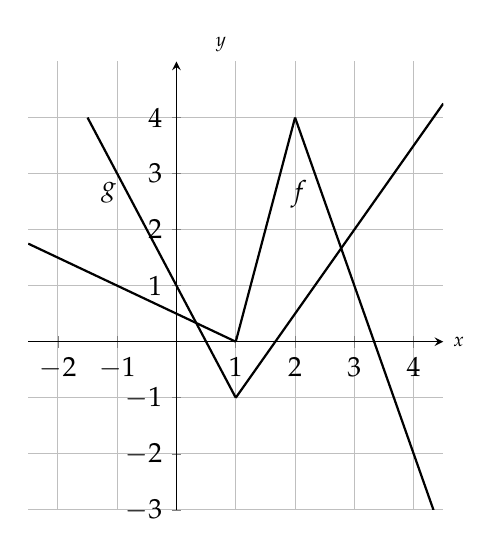
\begin{tikzpicture}
\begin{axis}[axis y line=middle,axis x line=middle, ymajorgrids=true, xmajorgrids=true, ymin=-3,ymax=5, xmin=-2.5,xmax=4.5, name=myplot, xscale=1/1.3, ytick={-3,-2,-1,0,1,2,3,4}]
\addplot [{\colorone}, domain=-1.5:1,thick] {-2*x+1}; 
\addplot [{\colorone}, domain=1:4.5,thick] {1.5*x-2.5};
\addplot [{\colortwo}, domain=-2.5:1, thick] {-.5*x+.5};
\node[label={30:{$g$}}] at (axis cs:-1.6,2.2) {};
\addplot [{\colortwo}, domain=1:2, thick] {4*x-4};
\node[label={30:{$f$}}] at (axis cs:1.6,2.1) {};
\addplot [{\colortwo}, domain=2:4.5, thick] {-3*x+10};
\end{axis}
\node [right] at (myplot.right of origin) {\scriptsize $x$};
\node [above] at (myplot.above origin) {\scriptsize $y$};
\end{tikzpicture}
\vskip .25 truecm
You can write this as 4 separately numbered problems, instead of 4 parts of one problem, if it works better that way.\\ 
(a) $(f \circ g)'(-1)$  \hskip .25 truecm (b) $(g \circ f)'(0)$ \hskip .25 truecm (c) $(g \circ g)'(-1)$ \hskip .25 truecm (d) $(f \circ f)'(4)$ \\

\indent Answers: (a) $(f \circ g)'(-1)=6$  \hskip 1 truecm (b) $(g \circ f)'(0)=1$ \hskip 1 truecm (c) $(g \circ g)'(-1)=-4$ \hskip 1 truecm (d) $(f \circ f)'(4)=1.5$ \\
\vskip .5 truecm

\vskip .5 truecm

\bgroup
\def\arraystretch{1.25}
 \begin{tabular}
{m{1cm}| m{1cm} | m{1cm} | m{1cm}| m{1cm}} 
 $x$ &  $f(x)$ & $f'(x)$ & $g(x)$ & $g'(x)$ \\  
\hline
 1 &  4 & 5 & 4 & 5 \\ 
 \hline
 4 &  0 & 7 & 1 & $\frac{1}{2}$\\
 \hline
 6 & 6 & 4 & 6 & 3\\  
\end{tabular}
\egroup\\
%I Need to figure out how to center table entries


Use the given table of values for $f, g, f', \text{and} g'$ to find\\
(a) $(f \circ g)'(6)$\\

\indent Answers: (a) $(f \circ g)'(6)=12$  \hskip 1 truecm (b) $(g \circ f)'(1)=2.5$ \hskip 1 truecm (c) $(g \circ g)'(6) =9$ \hskip 1 truecm (d) $(f \circ f)'(1)=35$ \\
\vskip .5 truecm


\tiny
\begin{flalign*}
\begin{aligned}
&= \displaystyle{ \frac{\ln x^2 [x \cdot \frac{d}{dx}(\cos (x^{-2})) + \frac{d}{dx}(x)\cdot (\cos (x^{-2})) -2 \sin e^{4x} \cdot \frac{d}{dx}(\sin e^{4x})] - \frac{d}{dx}(\ln x^2) \cdot [x\cos (x^{-2}) -\sin^2(e^{4x})]}{(\ln x^2)^2}}\\
\\
&= \displaystyle{ \frac{(\ln x^2) [x(-\sin (x^{-2})\cdot \frac{d}{dx}(x^{-2})) + 1 (\cos (x^{-2})) -2 \sin e^{4x} \cos e^{4x} \cdot \frac{d}{dx}(e^{4x})] - \frac{1}{x^2} \frac{d}{dx}(x^2) \cdot [x\cos (x^{-2}) -\sin^2(e^{4x})]}{(\ln x^2)^2}}\\
\\
&= \displaystyle{ \frac{(\ln x^2) [-x(\sin x^{-2})(-2x^{-3}) + 1\cdot (\cos (x^{-2})) -2 \sin e^{4x} \cos e^{4x} \cdot (4e^{4x})] - \frac{1}{x^2} (2x) \cdot [x\cos (x^{-2}) -\sin^2(e^{4x})]}{(\ln x^2)^2}}\\
\\
&= \displaystyle{ \frac{(\ln x^2) [2x^{-2}(\sin x^{-2}) + (\cos (x^{-2})) - 8e^{4x} \sin e^{4x} \cos e^{4x} ] - 2x^{-1} [x\cos (x^{-2}) -\sin^2(e^{4x})]}{(\ln x^2)^2}}\\
\end{aligned}
\end{flalign*}
\normalsize
\vskip .5 truecm



\textbf{p. 85} \\
$\displaystyle{\frac{d}{dx}[f(x)g(x)] = 7x^6 \neq 10x^5.}$ 

Applying the \textbf{real} Product Rule we see that,
\begin{flalign*}
\begin{aligned}
\displaystyle{\frac{d}{dx}[f(x)g(x)]} & = \displaystyle{x^2 \frac{d}{dx} (x^5) + \frac{d}{dx} (x^2) \cdot x^5}\\ 
& = x^2 \cdot 5x^4+2x \cdot x^5 \\ 
&= 7x^6\\
\end{aligned}
\end{flalign*}
\vskip .5 truecm

\small   
\begin{flalign*}
\begin{aligned}
\displaystyle{\frac {d}{dx} \left(\frac {f(x)}{g(x)}\right)} &= \displaystyle{\lim_{h\to 0}} \frac{\frac {f(x+h)}{g(x+h)} - \frac {f(x)}{g(x)}}{h}, ~~\text{where}~ h \neq 0\\
\\
&= \displaystyle{\lim_{h\to 0}} \left[ \left( \frac {f(x+h)}{g(x+h)} - \frac {f(x)}{g(x)}\right) \cdot \frac {1}{h}\right]\\ 
\\
&=\displaystyle{\lim_{h\to 0}} \left[ \left( \frac {f(x+h)g(x) - f(x)g(x+h)}{g(x+h)g(x)}\right) \cdot \frac {1}{h}\right]\\
\end{aligned}
\end{flalign*}
\normalsize  %%%%%Switch back to normal size.

Example 54 solution insert the details of quotient rule in the first step:\\

$\displaystyle{\frac {d}{dx} \left(\frac {5x^2}{\sin x}\right) = \frac{\sin x \frac{d}{dx}(5x^2) - 5x^2 \frac{d}{dx}(\sin x)}{(\sin x)^2}}$
\vskip 1 truecm

Similarly for Example 55 insert a second step:\vskip .25 truecm
$\displaystyle {= \frac{\cos x \frac{d}{dx}(\sin x) - \sin x \frac{d}{dx} (\cos x)}{(\cos x)^2}}$
\vskip 1 truecm

Last line: \sout{The Quotient Rule gives...} and replace it with:\\
When we stated the Power Rule in Section $2.3$ we claimed that it worked for all $n \in \mathbb{R}$ but only provided the proof for $n \in \mathbb{Z}^+$. \\
\vskip 1 truecm


\textbf{Answers}:\\

7. \begin{flalign*}
\begin{aligned}
\displaystyle{\frac{d}{dx}(\cot x)} &= \displaystyle{\frac{d}{dx}\left(\frac{\cos x}{\sin x}\right)}\\ &= \displaystyle{\frac{\sin x (-\sin x) - (\cos x)(\cos x)}{(\sin x)^2}}\\
&= \displaystyle{\frac{-[(\sin x)^2 + (\cos x)^2]}{(\sin x)^2}}\\
&= \displaystyle{\frac{-1}{(\sin x)^2}} = -\csc^2 x\\
\end{aligned}
\end{flalign*}
\vskip .5 truecm


\textbf{After \#21:} \\
\indent $\displaystyle{g(x)=\frac{1}{1+x+x^2+x^3}}$\vskip .5 truecm
\indent $\displaystyle{p(x)=1+\frac{1}{x}+\frac{1}{x^2}+\frac{1}{x^3}}$\vskip .5 truecm

\begin{tikzpicture}
\begin{axis}[tick label style={font=\scriptsize},minor x tick num=1,axis y line=middle,axis x line=middle,ymin=-3,ymax=2,xmin=-.5,xmax=3.5,name=myplot, xscale=1/1, scale=.65]
\addplot [domain=-0.5:3.5] {-x*(x-2)};
\end{axis}
\node [right] at (myplot.right of origin) {\scriptsize $x$};
\node [above] at (myplot.above origin) {\scriptsize $y$};
\end{tikzpicture}
\vskip .5 truecm

\textbf{Proof: Differentiation Power Rule when $n$ is a positive integer}\vskip .25 truecm
Let $f(x)= x^n$, where $n \in \mathbb{Z}^+$. By the definition of derivative,\\
\small    %%%%%%  Changes text size - makes things fit better.%%%%%%%%%%%
\begin{flalign*}
\begin{aligned}
f'(x) &= \displaystyle{\lim_{h\to 0}} \frac{(x+h)^n - x^n}{h}, ~~\text{where}~ h \neq 0\\
&= \displaystyle{\lim_{h\to 0}} \frac{(x+h)^n - x^n}{h}, ~~\text{use the Binomial Theorem to expand\ } (x+h)^n\\  %%%Changed where this comment is and then there is only one align environment.  
&=\displaystyle{\lim_{h\to 0}} \frac{x^n + \binom{n}{1} hx^{n-1} + \binom{n}{2} h^2x^{n-2}+ ... +\binom{n}{n-1} h^{n-1}x + \binom {n}{n} h^n)   -x^n}{h},\\
\end{aligned}
\end{flalign*}
\normalsize  %%%%%Switch back to normal size.
\vskip .5 truecm

\begin{center} $g(x) = x^6 + 3x^4 + 3x^2 + 1$ \end{center}
\vskip .25 truecm

new\#32 The figure shows the graphs of $f, f', f''$ and $f'''$. Identify each curve and explain your choices.\\

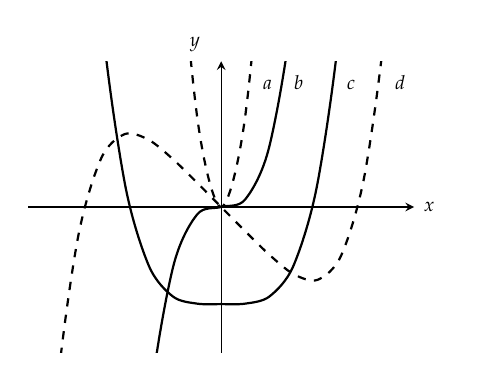
\begin{tikzpicture}
\begin{axis}[xtick=\empty, ytick=\empty, axis y line=middle,axis x line=middle, ymin=-3,ymax=3, xmin=-2,xmax=2, name=myplot, xscale=1.1/1, scale=.65]
\addplot [{\colorone}, dashed, smooth, domain=-3:3,thick] {.5*x^5-2*x}; 
\node[label={30:{\scriptsize $a$}}] at (axis cs:.23,2.1) {};
\addplot [{\colortwo}, smooth, domain=-3:3,thick] {2.5*x^4-2};
\node[label={30:{\scriptsize $b$}}] at (axis cs:.55,2.1) {};
\addplot [{\colorone}, smooth, domain=-3:3, thick] {10*x^3};
\node[label={30:{\scriptsize $c$}}] at (axis cs:1.1,2.1) {};
\addplot [{\colortwo}, dashed, smooth, domain=-3:3, thick] {30*x^2};
\node[label={30:{\scriptsize $d$}}] at (axis cs:1.6,2.1) {};
\end{axis}
\node [right] at (myplot.right of origin) {\scriptsize $x$};
\node [above] at (myplot.above origin) {\scriptsize $y$};
\end{tikzpicture}
\vskip .5 truecm

new \#21. Sketch the graph of the function $h$ for which $h(1)=0, h'(1)>0, h'(2)=0,$ and $h'(3)>0$. 

39. (a) $v(t) = 4t^3 - 8t, ~ a(t)=12t^2 - 8$\\
\indent (b) $a(1.5) = 19~ \text{ft/s}^2$\\  
\indent (c) $t=0$ sec and $t=\sqrt{\frac{3}{2}}$ sec
\vskip .25 truecm

\end{document}